Si danno per assunte tutte le conoscenze relative alla teoria delle code viste nel corso di Telecomunicazioni. Per ulteriori dettagli, si veda~\cite[cap. 8]{libro:tele}.
Per una facile comprensione, vengono riportate di seguito delle nozioni riguardanti la blockchain, le criptovalute e le catene di Markov.

\section{Blockchain e criptovalute}
\label{sottocap:bc-cripto}
La \textit{\textbf{blockchain}} \`e un registro pubblico, condiviso e decentralizzato che non permette la falsificazione delle informazioni registrate (chiamate anche \textit{transazioni} o \textit{entry}). Queste informazioni, sono raggruppate in \textit{blocchi}, collegati tra loro in ordine cronologico. L'insieme di tutti questi blocchi, forma l'intero registro (ledger).
La rete blockchain viene realizzata configurando un \textit{sistema peer-to-peer}. Essa \`e un tipo di rete in cui i nodi (o peer) possono comunicare e condividere risorse tra loro, senza dover passare per un'autorità centrale (come un server). Quest'ultima proprietà, \`e detta \textit{decentralizzazione}.\\
Una \textit{\textbf{criptovaluta}} \`e un sistema di scambio digitale peer-to-peer in cui vengono utilizzate tecniche crittografiche per generare e spedire unità di valuta~\cite{art:bc2}. Dunque, essa implementa un sistema blockchain, in cui i dati registrati sono transazioni finanziarie. In parole povere, una criptovaluta \`e una moneta digitale che ha un valore di mercato come una moneta fisica.
Le criptovalute più conosciute e utilizzate sono: \textit{Bitcoin}, \textit{Ethereum} e \textit{Monero}.

%**************************************************************
\subsection{Transazioni}
In una blockchain di criptovalute, le \textit{transazioni} sono quelle informazioni pubbliche associate al trasferimento di criptovalute tra partecipanti nel sistema. 
Ogni transazione non \`e collegata alla sua precedente in ordine cronologico, ma alla sua \textit{transazione-input}, ovvero al precedente scambio, o ai precedenti scambi, che hanno fornito delle criptovalute al ricevente così da poter diventare ora il mittente nella transazione in questione~\cite{tesi:venezia}.
Le transazioni possono essere di diversi tipi:~\cite{libro:bitcoin}
\begin{itemize}
\item \textit{Transazioni con resto}: quando si ha un input e due output. Nel mondo reale, sono l'equivalente dell'acquisto di un bene in cui l'acquirente riceve un resto.
\item \textit{Transazioni aggregatrici}: quando si hanno più input ed un solo output. Nel mondo reale, sono l'equivalente dello scambiare una pila di monete per una banconota singola di valore maggiore.
\item \textit{Transazioni distribuite}: quando si ha un solo input e più output. Nel mondo reale, sono l'equivalente del pagamento da parte di uno stesso pagatore a più riceventi, in una sola operazione; ad esempio quando un'azienda paga gli stipendi a tutti i suoi dipendenti.
\end{itemize}

%**************************************************************
\subsection{Crittografia alla base di una criptovaluta}
Ogni utente della rete possiede: 
\begin{itemize}
\item un portafoglio (wallet) contenente chiavi crittografiche private, generate di volta in volta quando avviene una transazione. 
\begin{itemize}
\item il \textit{wallet} \`e l'equivalente di un portafoglio materiale, che contiene la coppia di chiavi pubblica e privata e mostra il proprio conto. Però, questo quantitativo di criptovalute, non \`e fisicamente posseduto nel proprio pc o su un server come se fosse una banca, ma \`e il risultato degli input e output registrati nelle transazioni salvate nella blockchain. 
\item la \textit{chiave privata} \`e una stringa alfanumerica segreta, generata e gestista dal software del wallet.
\end{itemize}
\item un \textit{indirizzo pubblico}, calcolato a partire dalla chiave crittografica pubblica tramite una funzione di hashing. Questo indirizzo serve per ricevere le transazioni. Gli indirizzi iniziano con i caratteri 1 o 3.
\begin{itemize}
\item la \textit{chiave pubblica} \`e una stringa alfanumerica visibile a tutti, generata e gestista dal software del wallet. Essa viene ricavata matematicamente dalla chiave privata. 
\item la \textit{funzione di hashing} \`e una funzione matematica che non \`e invertibile e mappa dati di qualsiasi lunghezza in stringhe di bit di lunghezza fissa (chiamate \textit{hash} o \textit{impronte}). Le funzioni di hash inoltre sono veloci da calcolare e resistenti alle collisioni perch\`e se si cambia anche un solo bit in ingresso, l’output viene stravolto (dunque \`e garantita l'integrità dei dati). Inoltre, essendo una funzione non invertibile, \`e altamente improbabile ottenere il dato di ingresso avendo a disposizione il suo hash.
\end{itemize}
\end{itemize}
Le chiavi crittografiche sono importanti perch\`e sono alla base della \textit{firma digitale}, lo strumento che garantisce sia l’autenticazione del mittente sia l’integrità dei dati. 
La firma digitale su un documento consiste nel cifrare il documento tramite la chiave privata e utilizzare la relativa chiave pubblica, che \`e nota a tutti, per decifrare la firma e quindi constatare o meno l’identità del mittente.
Ogni proprietario trasferisce le criptovalute firmando digitalmente l’hash della transazione precedente (quella che viene chiamata transazione-input) e la chiave pubblica del futuro proprietario, e aggiungendo queste informazioni alla transazione corrente~\cite{art:satoshi}. In questo modo, le transazioni sono legate tra loro e quando un utente vuole spendere le sue criptovalute (quindi fare una nuova transazione), dovrà ``sbloccare" la catena fornendo la sua chiave pubblica. 
Attraverso la presentazione della chiave pubblica e della firma, tutti i membri della rete possono decifrare la firma con la chiave pubblica del mittente e verificare che l’hash risultante corrisponde all’impronta digitale di quella transazione. Di conseguenza:
\begin{itemize}
\item la transazione \`e valida e integra (la firma \`e infatti legata all’impronta digitale e quindi alla transazione stessa. Una modifica della transazione produrrebbe un’impronta digitale totalmente diversa);
\item l'identità del mittente \`e autentica.
\end{itemize}
Questo processo di verifica e autenticazione \`e mostrato nella fig.~\ref{im:verifica}
\begin{figure}[!h]
\centering 
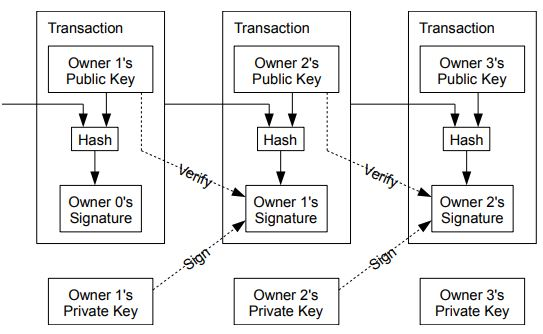
\includegraphics[scale=0.75]{immagini/cap2/1-autenticazione} 
\caption{Autenticazione della catena di transazioni}
\label{im:verifica} 
\end{figure}

%**************************************************************
\subsection{Struttura dei blocchi}
Come dice il nome, la blockchain \`e una catena di blocchi, contenenti transazioni valide. L'intera rete \`e formata da utenti chiamati \textit{nodi}, che possono essere localizzati in qualsiasi parte del pianeta. Ciascun nodo contiene il registro di tutte le transazioni effettuate nella rete fino a quel momento.
Un qualsiasi blocco contiene le seguenti informazioni~\cite{art:bc2}:
\begin{itemize} 
\item la dimensione (in byte) del blocco;
\item l'\textit{intestazione} (header) con diversi campi al suo interno, mostrati nella tab.~\ref{tab:intestazione};
\item il numero totale di transazioni. 
Ogni blocco \`e identificato in maniera univoca da un \textit{hash}, generato usando l’algoritmo crittografico di hashing sull’intestazione del blocco (per il Bitcoin, per esempio, l'algoritmo \`e SHA-256). La tab.~\ref{tab:blocco} mostra la struttura di un blocco.
\end{itemize}
\begin{table}
\centering
\begin{tabular}[t]{|c|l|}
\hline
\textbf{Campo} & \textbf{Descrizione} \\
\hline
Previous Block Hash & Hash del blocco precedente (parent block) a cui \`e collegato\\
\hline
Merkel Root & Hash della radice del merkel tree associato al blocco \\
\hline
Timestamp & Ora di creazione del blocco \\
\hline
Difficulty Target & Target usato per il PoW \\
\hline
Nonce & Numero contatore usato per il PoW \\
\hline
\end{tabular}
\caption{Struttura dell'intestazione}
\label{tab:intestazione}
\end{table}
\begin{table}
\centering
\begin{tabular}[t]{|c|l|}
\hline
\textbf{Campo} & \textbf{Descrizione} \\
\hline
Block Size & Dimensione del blocco in bytes \\
\hline
Block Header & Intestazione del blocco contenente diversi campi \\
\hline
Counter & Numero totale di transazioni registrate \\
\hline
Transactions & Transazione registrate nel blocco \\
\hline
\end{tabular}
\caption{Struttura di un blocco}
\label{tab:blocco}
\end{table}
I blocchi sono collegati ``all'indietro" (back-linked), cio\`e ognuno si riferisce al blocco precedente presente nella catena. Per questo motivo, la blockchain \`e spesso visualizzata come una pila verticale, con blocchi stratificati l’uno sopra l’altro. Questa visualizzazione, provoca l’uso di terminologie come \textit{altezza} (height) per riferirsi alla distanza dal primo blocco e \textit{top} o \textit{tip} (cima o punta) per riferirsi al blocco aggiunto più recentemente.
Ciascun blocco inoltre referenzia il blocco precedente, conosciuto anche come \textit{parent block} (blocco genitore), attraverso il campo \textit{previous block hash} dell'intestazione. La sequenza di hash che collegano ogni blocco al proprio genitore crea una catena che si collega, blocco per blocco fino al primo blocco creato, denominato \textit{genesis block}.
Una semplice rappresentazione \`e mostrata nella fig.~\ref{im:pila}.
\begin{figure}
\centering 
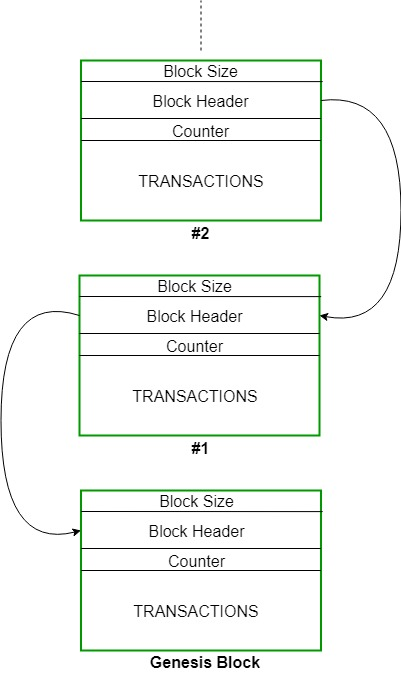
\includegraphics[scale=0.65]{immagini/cap2/2-BC-come-catena} 
\caption{Blockchain vista come una catena}
\label{im:pila} 
\end{figure}
Si supponga che un genitore venga modificato in qualsiasi modo. Allora il suo hash cambia. L’hash modificato necessita un cambio nel puntatore \textit{previous block hash} del figlio. Questo, a sua volta, causa il cambio dell’hash del figlio, che richiede il cambio nel puntatore dell’hash nipote, che a sua volta cambia il puntamento al nipote, e così via. Questo effetto a cascata assicura che, fino a quando un blocco ha tante generazioni di blocchi che lo seguono, non può essere modificato senza forzare un ricalcolo su tutti i blocchi seguenti. Visto che per questo ricalcolo servirebbe un’enorme potenza computazionale, l’esistenza di una lunga catena di blocchi fa sì che la storia più profonda della blockchain sia immutabile, che \`e una degli elementi chiave della sicurezza della blockchain~\cite{libro:bitcoin}.

%**************************************************************
\subsection{Funzionamento}
Le nuove transazioni devono per prima cose essere confermate, cio\`e bisogna verificare la loro firma digitale. Questo procedimento, lo possono fare tutti gli utenti della rete. La firma digitale, però, non offre protezione contro il \textit{double spending}, cio\`e quando un utente spende più volte delle criptovalute già spese~\cite{art:satoshi}. Per risolvere questo problema, bisogna tener conto anche dei vecchi blocchi (e quindi delle vecchie transazioni), e provare che quelli nuovi, sono legati matematicamente ai precedenti. Siccome questa verifica deve essere rigorosa e non esiste un'autorità centrale, il compito spetta ai nodi della rete (lo possono fare tutti o solo alcuni). Questi nodi specializzati, prendono il nome di \textit{minatori} (o miner) e il processo di verifica che eseguono si chiama \textit{mining}. Esso può essere diverso da criptovaluta a criptovaluta. La conferma avviene trovando il valore di hash che soddisfa una certa proprietà (procedimento chiamato \textit{proof of work}, abbreviato \textit{PoW}). Quando si trova una soluzione, il nuovo blocco \`e ritenuto valido e viene aggiunto al registro di ogni nodo. Il risultato finale \`e una catena di blocchi approvati non modificabili e in ordine cronologico.

%**************************************************************
\subsection{Mining di una criptovaluta}
Per \textit{mining} si intende quel processo svolto da un insieme di utenti della rete che, fa eseguire all'hardware di ogni utente calcoli matematici al fine di confermare il nuovo blocco ed aumentare la sicurezza della rete~\cite{sito:bitcoin}.
Questo processo ha due scopi:
\begin{itemize}
\item mantiene l’integrità e l’autenticità della blockchain, assicurando che le transazioni siano confermate solo se \`e stata usata sufficiente potenza di calcolo per il blocco che le contiene;
\item emette una quantità stabilita di nuove criptovalute (quasi come una banca centrale emette nuova moneta), che spettano al minatore che per primo le ha prodotte. A tale quantità prestabilita va a sommarsi anche il totale delle commissioni delle transazioni registrate nel blocco~\cite{art:bc2}.
\end{itemize} 
Dunque, la sicurezza della blockchain \`e resa possibile da quanti più nodi “onesti” sono presenti nella rete, in modo da rendere difficile (se non impossibile) il lavoro dei nodi “disonesti” che vogliono invece modificare il registro a loro vantaggio. 
L’onestà dei nodi \`e ``comprata” attraverso un particolare sistema di attribuzione di ricompense, che incentivano tale onestà~\cite{tesi:venezia}.
Quando arrivano delle nuove transazioni, esse vengono aggiunte a un pool temporaneo di transazioni non verificate. Questo pool, \`e memorizzato da ogni minatore. Man mano che i minatori generano un nuovo blocco, prelevano le transazioni non verificate dal pool. Esse vengono aggiunte al nuovo blocco, ordinate secondo certi criteri (ad esempio, dando priorità a quelle con commissioni maggiori). Da qui in poi, ogni minatore inizia il processo di mining di un nuovo blocco di transazioni. Nel momento in cui riceve un blocco valido da un altro minatore, capisce di aver perso la sfida. Dunque lo controlla (procedimento chiamato \textit{consenso}) e lo aggiunge alla sua blockchain. Dopodich\`e, ritenta la sfida con un nuovo blocco, creato a partire da altre transazioni e il procedimento si ripete.
Più nel dettaglio, il funzionamento del processo di mining \`e il seguente: il minatore ha come input l'intestazione del blocco nuovo e un numero, chiamato \textit{nonce} (che, tra l'altro, \`e un campo presente nell'intestazione). Il nonce \`e un numero (spesso scelto arbitrariamente) che viene utilizzato solo una volta per questo scopo e poi scartato~\cite{art:bc1}. L'input \`e rappresentato nella fig~\ref{im:input}.
\begin{figure}
\centering 
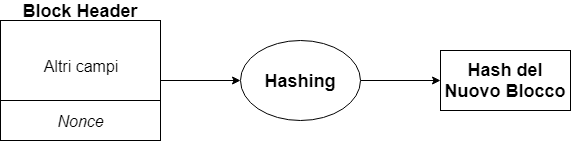
\includegraphics[scale=0.55]{immagini/cap2/3-input} 
\caption{Input utilizzato per il calcolo dell'hash del nuovo blocco}
\label{im:input} 
\end{figure}
Ora, partendo da questo input, il minatore calcola il corrispettivo hash e verifica se ha una certa proprietà/struttura definita dalla criptovaluta. Se così non fosse, cambia nonce e ritenta. Il compito del minatore, \`e dunque quello di trovare il nonce che soddisfa la proprietà. L'insieme di questi compiti matematici, prende il nome di \textit{proof of work}, abbreviato in \textit{PoW} (prova del lavoro).
La complessità del proof of work sta proprio nell'ottenere il nonce corretto, in quanto questo comporta il calcolo di un numero esponenziale di hash~\cite{art:bc2}.
Una volta che un minatore trova la soluzione per validare il blocco, manda a tutti gli altri minatori della rete:
\begin{itemize}
\item il nuovo blocco appena confermato;
\item il nonce corretto;
\item l'hash del nuovo blocco (calcolato con il nonce corretto), che \`e legato all'ultimo blocco, in quanto, per calcolarlo, \`e stato utilizzato il suo hash.
\end{itemize}
Essi, dovranno confermare che il risultato trovato \`e corretto. Se \`e così, il nuovo blocco viene aggiunto ``in cima" alla blockchain e il minatore che ha validato il blocco per primo otterrà la ricompensa. Tale verifica, chiamata anche \textit{consenso}, \`e semplice e veloce, in quanto basta calcolare un solo hash e verificare che combaci~\cite{art:bc2}.

%**************************************************************
\subsection{Numero di conferme}
Nella realtà, succede molto spesso che i minatori scelgono transazioni diverse per un blocco (scegliendo, per esempio, quelle con commissioni elevate). Quindi ognuno può lavorare su un potenziale blocco diverso che cercherà di confermare prima degli altri. Quello che succede in questo caso, \`e che si formino delle \textit{ramificazioni} nella parte finale della blockchain. Quando avvengono queste situazioni, la soluzione da adottare \`e specificata negli algoritmi delle criptovalute. Una regola molto comune, \`e quella di far continuare la blockchain sul suo ramo più lungo, mentre tutto il resto viene ignorato. Nella fig.~\ref{im:rami} \`e mostrato un esempio di blockchain ramificata, che continua sul ramo più lungo.
\begin{figure}
\centering
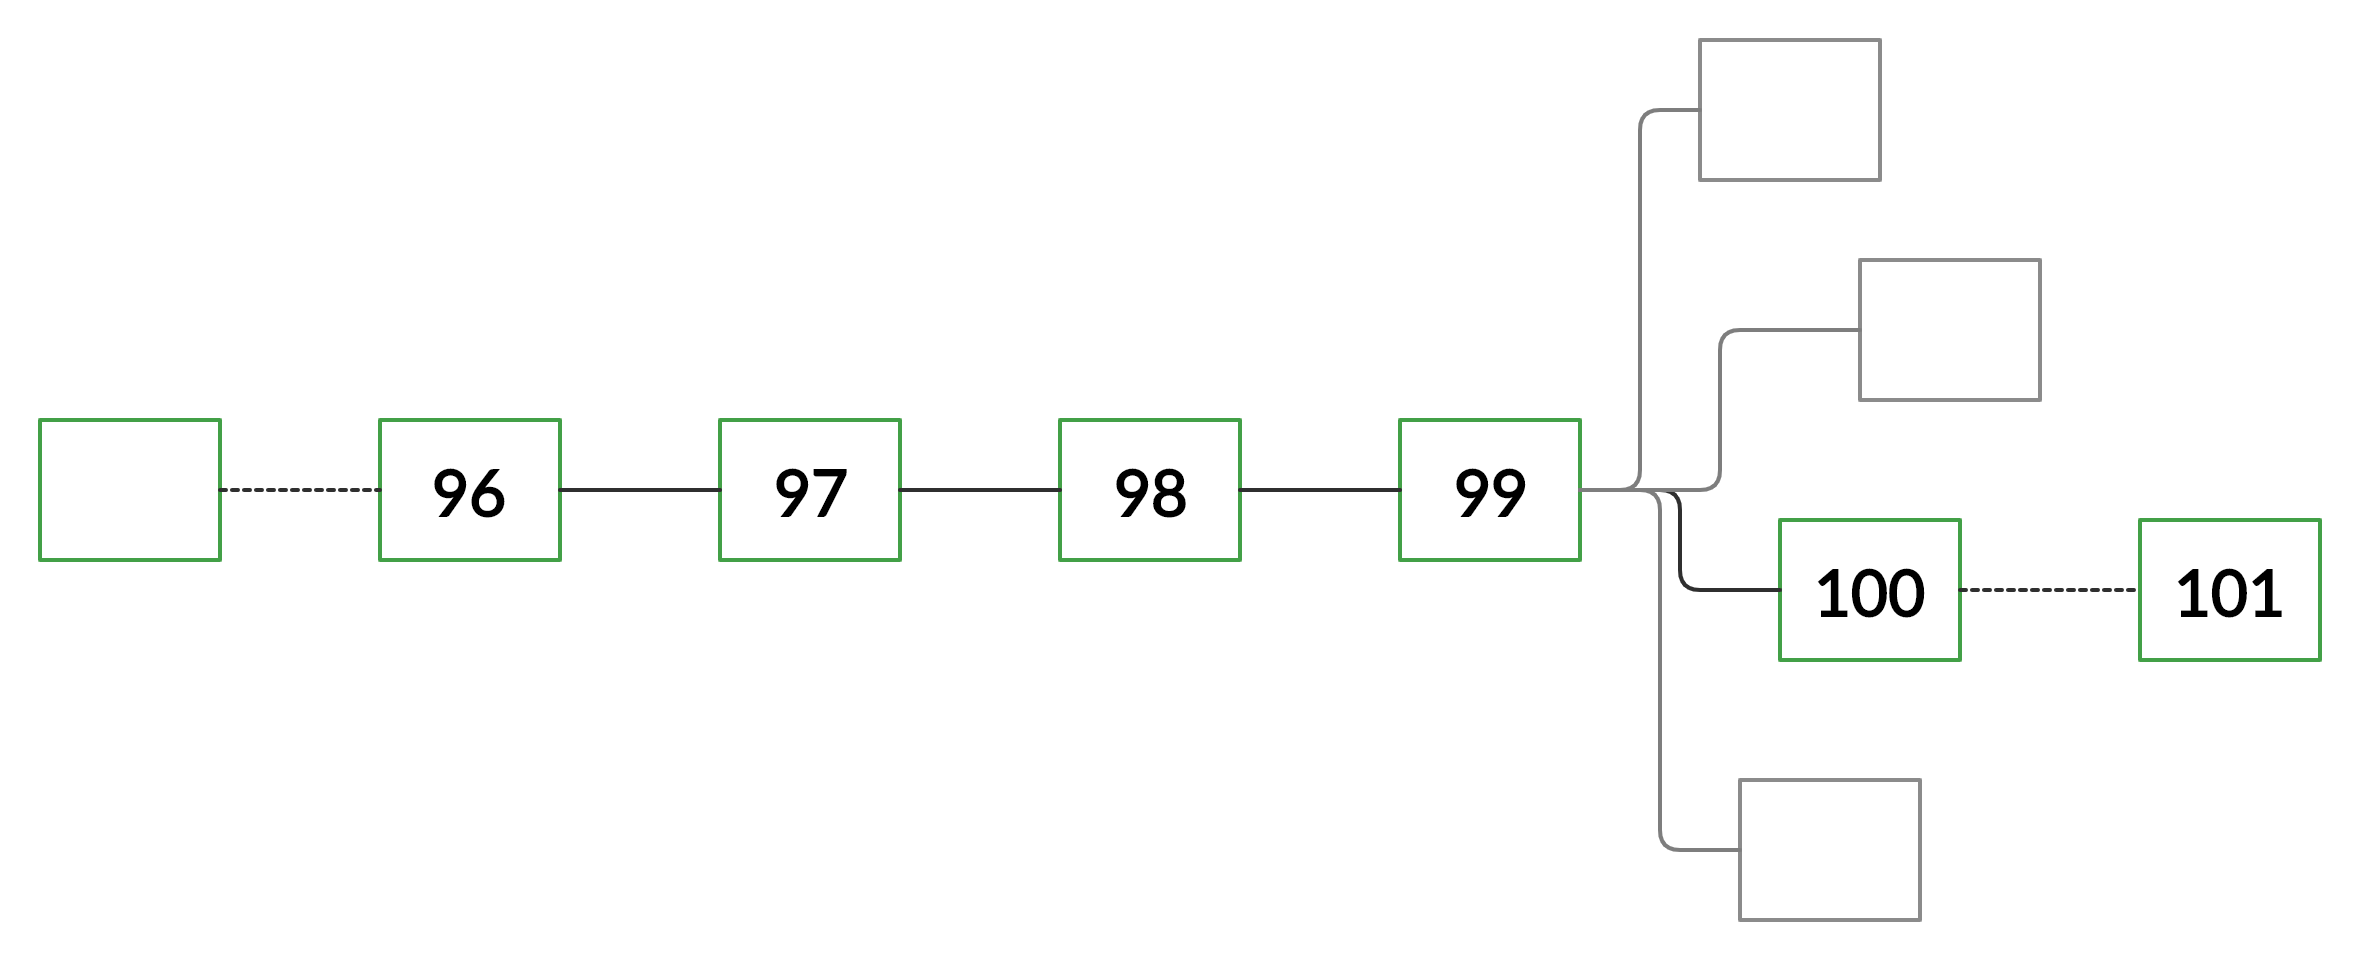
\includegraphics[scale=0.18]{immagini/cap2/3-rami} 
\caption{Esempio di blockchain ramificata}
\label{im:rami} 
\end{figure}
Basandoci sulla fig.~\ref{im:rami}, supponiamo che l’ultimo blocco confermato della blockchain sia il blocco numero 100. Ora, supponiamo che un minatore malintenzionato voglia contraffare questo blocco e quindi lo modifichi. Ovviamente, potrà apporre tale modifica solo sulla copia della blockchain che ha sul suo server. Dopodich\`e, dovrà far accettare (e quindi divulgare) la sua copia “contraffatta” al resto della rete.
Per riuscire nel suo intento, il malintenzionato dovrà:
\begin{itemize}
\item trovare un nonce per il blocco 100 che lui ha modificato, in modo che il sistema non evidenzi il suo tentativo di contraffazione;
\item aggiudicarsi la gara sul blocco 101 (perch\`e si continua sul ramo più lungo). 
\end{itemize}
In sostanza, dovrà riuscire a trovare 2 nonce (per il blocco 100 e blocco 101) prima che un qualunque altro minatore riesca a trovarne uno solo, ovvero quello per il blocco 101. 
Il tutto sarà esponenzialmente più improbabile se vorrà contraffare una transazione del blocco 99 perch\`e dovrà trovare tre nonce\dots\, e così via per i blocchi precedenti.
Per questi motivi, per misurare la sicurezza di una transazione, si indicano il numero delle conferme che ha ricevuto: ad esempio, se l’ultimo blocco confermato \`e il numero 100, allora una transazione presente nel blocco 98 si dice abbia 3 conferme, ovvero la conferma del blocco 98, quella del 99 e quella del 100.

%**************************************************************
\subsection{Esempio: Mining del Bitcoin}
Il processo di mining di un Bitcoin si basa sull'algoritmo \textit{Hashcash}~\cite{art:satoshi}. Il funzionamento \`e molto simile a quello descritto in precedenza per una criptovaluta generale. In particolare, Bitcoin utilizza \textit{SHA-256} come funzione di hash (ciò significa che l'impronta generata sarà di 256 bit). Inoltre, il minatore deve trovare quel nonce tale per cui l'hash di output inizi con $n_z$ zeri, dove $n_z$ sono i bit più significativi~\cite{art:bc2}.
Per vedere se il nonce utilizzato \`e quello corretto, il minatore controlla se l'hash risultante \`e minore o uguale di un certo valore di 256 bit, chiamato \textit{target} (che tutti i minatori conoscono). Se \`e più piccolo, significa che l'output aveva almeno uno zero inziale in più rispetto al target e dunque il minatore ha trovato la soluzione; altrimenti, il nonce viene incrementato di uno e si riprova (il nonce parte da zero). Il valore target viene ricalcolato ogni 2016 blocchi (circa due settimane). Ad esempio, se il target corrente fosse di $00000111$ e l'hash di output $001110010$, il minatore non avrebbe trovato una soluzione valida, perch\`e il target ha 5 zeri iniziali e il risultato solo 2; il minatore deve aumentare progressivamente il nonce ad ogni nuovo tentativo, finch\`e il risultato non inizia con almeno 6 zeri~\cite{tesi:venezia}. La fig~\ref{im:flow} mostra il diagramma a blocchi del processo di mining del Bitcoin.
\begin{figure}
\centering
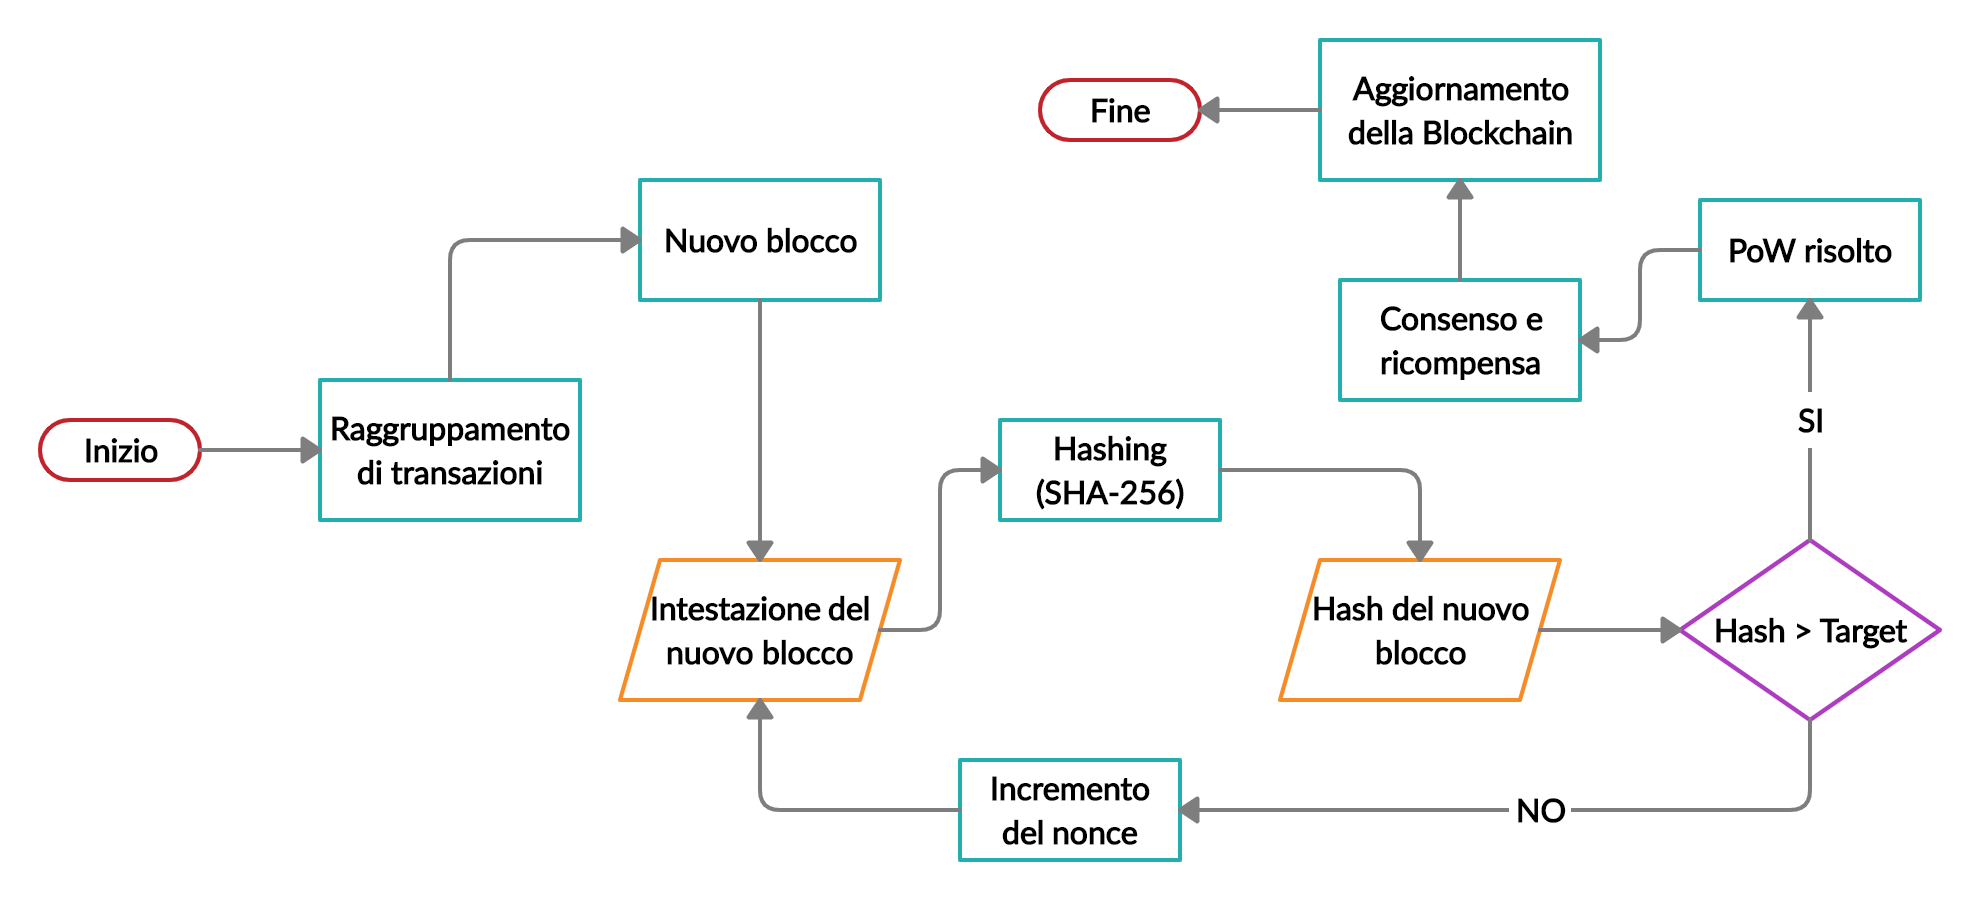
\includegraphics[scale=0.23]{immagini/cap2/4-flow} 
\caption{Diagramma a blocchi del processo di mining del Bitcoin}
\label{im:flow} 
\end{figure}
Il lavoro medio richiesto \`e esponenziale rispetto al numero di zeri. In più, SHA-256 richiede un \textit{hash rate}% 
\footnote{Per \textit{hash rate} si intende l'unità di misura della potenza di elaborazione della rete di una criptovaluta, cio\`e quanti calcoli matematici riesce ad eseguire in un certo tempo. Ad esempio, quando la rete raggiunge un hash rate di 10 TH/s, significa che può realizzare un trilione di calcoli al secondo.~\cite{sito:bitcoin}} elevato, di giga hashes al secondo (GH/s) o superiore~\cite{art:bc1}. 
Il tempo medio necessario per estrarre un blocco Bitcoin con SHA-256 \`e circa di 10 minuti~\cite{sito:bitcoin}.
Il procedimento di proof of work del Bitcoin \`e identico a quello descritto precedentemente per una criptovaluta generale.
Il minatore che ha risolto per primo il blocco, verrà premiato con dei Bitcoin. Il premio varia in base al numero di Bitcoin estratti. Poich\`e c'\`e n\`e un numero limitato, i premi diminuiscono della metà dopo ogni 210.000 blocchi estratti (circa ogni 4 anni). A partire da agosto 2018, i minatori vengono premiati con 12,5 Bitcoin. Nei primi anni, cio\`e nel 2009, i minatori guadagnavano 50 Bitcoin~\cite{art:bc2}.
Oltre alla ricompensa ottenuta dal mining, i minatori ricevono anche un importo chiamato \textit{commissione di transazione} per ogni transazione confermata che aggiungono alla blockchain~\cite{art:bc1}.
Per convenzione, una transazione che riceve 6 conferme (cio\`e sopra il suo blocco ne vengono aggiunti altri 5) viene considerata sicura al 100\%.



\section{Catena di Markov}
\label{sottocap:teo-code}
Una \textit{\textbf{catena di Markov}} \`e un processo stocastico avente una proprietà caratterizzante, chiamata \textit{proprietà di Markov}~\cite{libro:tele}.  Il processo, che può essere a tempo continuo o a tempo discreto, \`e determinato da una successione di variabili aleatorie $\{X_w\}$, che prendono valori in un insieme $S$, detto \textit{spazio degli stati}. Esso può essere finito o al più infinito numerabile. 
L’indice $w$ di $\{X_w\}$ indica il \textit{tempo}, mentre i possibili valori della successione prendono il nome di \textit{stati} del processo.
Al trascorrere del tempo, il processo può “saltare“ da uno stato all’altro. Se ad un certo istante $w$ si trova in uno stato $i$ ed all’istante successivo ($w+1$ se \`e discreto oppure $w+u$ se \`e continuo) si trova in uno stato $j \neq i$, si dirà che c’\`e stata una \textit{transizione}.
Siccome i processi coinvolti sono stocastici, i calcoli coinvolgeranno le probabilità. Le più importanti sono le cosiddette \textit{probabilità di transizione}. Per il \textit{tempo discreto} valgono:
\begin{equation}P_{i,j}(k)=P[X_{n+k}=j | X_n=i]\end{equation} 
che indica la probabilità di trovarsi nello stato $j$ al tempo $n+k$ sapendo di essere nello stato $i$ al tempo $n$. In questo caso, $k$ indica il \textit{numero di step} per andare dallo stato $i$ allo stato $j$.\\
Per il \textit{tempo continuo} invece, valgono:
\begin{equation}P_{i,j}(u)=P[X(t_0+u)=j | X(t_0)=i]\end{equation} 
che indica la probabilità di trovarsi nello stato $j$ al tempo $t_0+u$ sapendo di essere nello stato $i$ al tempo $t_0$. In questo caso, $u$ indica l'\textit{intervallo temporale} per andare dallo stato $i$ allo stato $j$.\\
Si dirà che queste probabilità sono $stazionarie$ se dipendono solo dalla lunghezza temporale $k$ o $h$ (a seconda che il tempo sia discreto o continuo) e non dai singoli istanti $n$ o $t_0$. Le relative catene di Markov, invece, si diranno \textit{omogenee}. I processi che si andranno a sviluppare nei capitoli successivi, sono tutti di questo tipo.

%**************************************************************
\subsection{Proprietà di Markov}
La proprietà di Markov per un processo a tempo discreto \`e sintetizzata nella seguente formula:
\begin{equation}\label{eq:pr1}P[X_{n_k}=\sigma_k | X_{n_{k-1}}=\sigma_{k-1},\dots,X_{n_0}=\sigma_0]=P[X_{n_k}=\sigma_k | X_{n_{k-1}}=\sigma_{k-1}].\end{equation}
Mentre, per un processo a tempo continuo, vale:
\begin{equation}\label{eq:pr2}P[X_{t_n}=\sigma_n | X_{t_{n-1}}=\sigma_{n-1},\dots,X_{t_0}=\sigma_0]=P[X_{t_n}=\sigma_n | X_{t_{n-1}}=\sigma_{n-1}],\end{equation}
dove i $\sigma_i$ sono elementi appartenenti allo spazio di stato $S=\{0,1,2,\dots\}$.\\
L’interpretazione della proprietà di Markov \`e la seguente. Consideriamo:
\begin{itemize}
\item l'istante $n_{k-1}$ (o nel continuo $t_{n-1}$) come il ``presente" del processo;
\item gli istanti $n_0, n_1, \dots, n_{k-2}$ (o nel continuo $t_0, t_1, \dots, t_{n-2}$) come il ``passato" del processo;
\item l'istante $n_k$ (o nel continuo $t_n$) come il ``futuro" del processo.
\end{itemize}
Dunque, le equazioni~\eqref{eq:pr1} e~\eqref{eq:pr2} ci dicono dice che la conoscenza del ``passato" del processo non predice la sua evoluzione futura dallo stato $\sigma_{k-1}$ in cui si trova al momento. Perciò, \`e possibile ``dimenticarsi" della storia passata, conoscendo esclusivamente lo stato presente.

